\documentclass{beamer}
\usetheme{Singapore}
\usepackage{tikz}
\usepackage{color}
\usetikzlibrary{positioning}
\usetikzlibrary{chains}
\usetikzlibrary{calc}
\usetikzlibrary{backgrounds}
%\usepackage{amsmath}
\title[Alba] % (optional, only for long titles)
{The Alba Storage System}
\subtitle{The \textcolor{red}{AL}ternative \textcolor{red}{BA}ckend}
\author[Slootmaekers, Doms] % (optional, for multiple authors)
{J.~Doms \and R.~Slootmaekers}
\institute[Open vStorage] % (optional)
{
%  \inst{1}%
%  Institute of Computer Science\\
%  University Here
%  \and
%  \inst{2}%
%  Institute of Theoretical Philosophy\\
%  University There
}
\date[Oct 2014] % (optional)
{Internal Presentation, 2014}
\subject{Alba}

\begin{document}
\frame{\titlepage}
\begin{frame}
  \frametitle{Requirements}
  \begin{itemize}[<+->]
     \item Object CR(U)D
     \item partial object retrieval
     \item optional encryption
     \item optional compression
     \item Namespaces($\star$)
     \item medium size deployments \pause (12 - 60 HDDs)
  \end{itemize}
\end{frame}

\begin{frame}
  \frametitle{Why not use \ldots}
  \framesubtitle{Swift/Ceph/DSS/\ldots}
  \begin{itemize}[<+->]
    \item{Swift?}
      \begin{itemize}
        \item via proxy server
        \item Replication (erasure coding `really soon now`)
        \item OSD: FS, object metadata = extended attribute.
        \item compression, encryption on the outside
        \item partial object retrieval!!
      \end{itemize}
    \item{Ceph?}
        \begin{itemize}
          \item via proxy server
          \item Replication (\& erasure coding since Q2 2014)
          \item OSD: FS (compression), encryption.
          \item partial object retrieval !?
        \end{itemize}
    \item{DSS?}
        \begin{itemize}
          \item via proxy server
          \item Erasure Coding (online codes)
          \item partial object retrieval ?!
          \item compression, encryption on outside.
        \end{itemize}
  \end{itemize}

\end{frame}
\begin{frame}
  \frametitle{Data flow}
  \framesubtitle{combining erasure coding, encryption and compression}
\begin{figure}
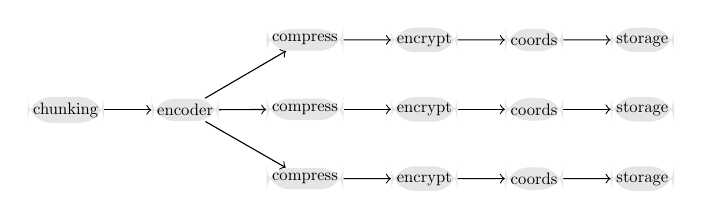
\begin{tikzpicture}[every node/.style={rectangle,fill=gray!20, rounded corners = 3mm}, scale = 0.60, transform shape]
  \node  (start) {chunking};
  \node  (encoder) [right=of start] {encoder};

  \node  (comp0)   [above right=of encoder] {compress};
  \node  (comp1)   [below=of comp0]   {compress};
  \node  (comp2)   [below=of comp1]   {compress};

  \node (encrypt0) [right=of comp0] {encrypt};
  \node (encrypt1) [right=of comp1] {encrypt};
  \node (encrypt2) [right=of comp2] {encrypt};

  \node (placement0) [right=of encrypt0] {coords};
  \node (placement1) [right=of encrypt1] {coords};
  \node (placement2) [right=of encrypt2] {coords};

  \node (storage0) [right=of placement0] {storage};
  \node (storage1) [right=of placement1] {storage};
  \node (storage2) [right=of placement2] {storage};
  \path[->] (start) edge (encoder)
            (encoder) edge (comp0)
            (encoder) edge (comp1)
            (encoder) edge (comp2)
            (comp0) edge (encrypt0)
            (comp1) edge (encrypt1)
            (comp2) edge (encrypt2)
            (encrypt0) edge (placement0)
            (encrypt1) edge (placement1)
            (encrypt2) edge (placement2)
            (placement0) edge (storage0)
            (placement1) edge (storage1)
            (placement2) edge (storage2);

\end{tikzpicture}
\end{figure}

\begin{equation*}
 crypt(zip(
     \begin{bmatrix}
     a_{1,1}  & a_{1,2}   & \ldots & a_{1,k} \\
     a_{2,1}  & \ldots    &        & a_{2,k} \\
     \ldots   & \ldots    & \ldots & \ldots  \\
     a_{k,1}  &  \ldots   &        & a_{k,k} \\
     \hline\\
     a_{k+1,1}& \ldots    & \ldots & a_{k+1,k} \\
     \ldots   &           &        & \ldots  \\
     a_{k+m,1}&           &        &
     \end{bmatrix} .
     \left[\begin{array}{c}x_{1}\\ x_{2}\\ \ldots \\ x_{k} \end{array}\right])
  )
 =
 \left[\begin{array}{c}
     b_{1} \\ b_{2} \\ \ldots \\ b_{k} \\
     \hline \\
     b_{k+1} \\ \ldots \\ b_{k+m} \end{array}
 \right]
\end{equation*}
partial retrieval $ \Rightarrow [a_{1,1},\ldots, a_{k,k}] = I$
\end{frame}

\begin{frame}
  \frametitle{Mark I architecture}
  \framesubtitle{ Alba Client LIB + Kinetic Drives }
 \begin{columns}[T] % contents are top vertically aligned
     \begin{column}[T]{5cm} % each column can also be its own environment
       \begin{figure}%[h!]
         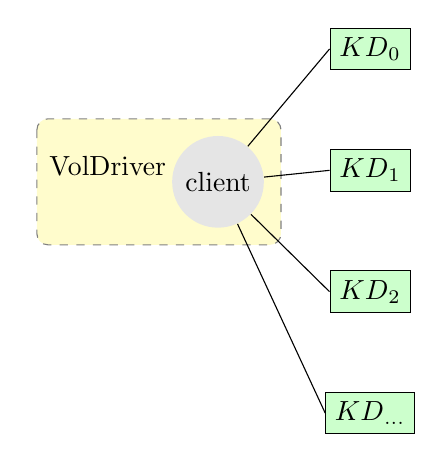
\begin{tikzpicture}
           \tikzset{
             my_data/.style={rectangle, fill=green!20, draw}
           }

           \node (client) [circle, fill=gray!20] {client};

           \node (osd0)  [my_data, above right = of client] {$\text{KD}_0$};
           \node (osd1)  [my_data, below = of osd0]        {$\text{KD}_1$};
           \node (osd2)  [my_data, below = of osd1]        {$\text{KD}_2$};
           \node (osdX)  [my_data, below = of osd2]        {$\text{KD}_{\ldots}$};

           \path[draw, -]
           (client) to (osd0.west)
           (client) to (osd1.west)
           (client) to (osd2.west)
           (client) to (osdX.west)
           ;

           \begin{pgfonlayer}{background}
             \path (client) + (-2.3,  0.8) node (a) {};
             \path (client) + (+0.8, -0.8) node (b) {};
             \path (client) + (+0.8, -0.8) node (c) {};
             \path[fill=yellow!20,rounded corners, draw=black!50, dashed]
             (a) rectangle (c);
             \path (client)+(-1.4,0.2) node (a) { VolDriver };
           \end{pgfonlayer}

         \end{tikzpicture}
       \end{figure}
     \end{column}
     \begin{column}[T]{5cm} % alternative top-align that's better for graphics
       \pause
       \begin{block}{But...}
       \begin{itemize}[<+(1)->]
         \item Kinetic client lib incompatible with VolDriver.
         \item VolDriver doesn't like \emph{eventual consistency}
       \end{itemize}
       \end{block}
     \end{column}
     \end{columns}
\end{frame}
\begin{frame}
\frametitle{Mark II architecture}
  \framesubtitle{ (Alba Client = Proxy) + Namespace Manager \& Kinetic Drives }
  \begin{columns}[T]
    \begin{column}[T]{5cm}
      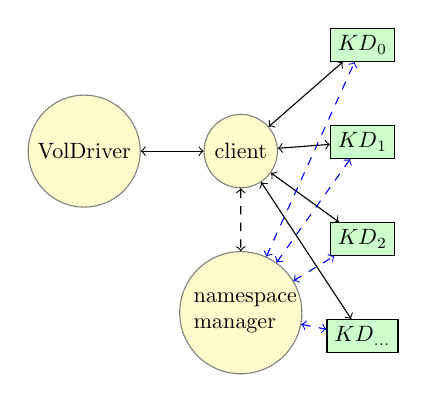
\begin{tikzpicture}[scale = 0.8, transform shape]
        \tikzset{
          my_data/.style={rectangle, fill=green!20, draw},
          my_process/.style={circle, draw = black!50, fill= yellow!20}
        }

        \node (client) [my_process] {client};
        \node (vd)     [my_process, left = of client] {VolDriver};
        \node (nm)     [my_process,
                        below = of client,
                        text width=1.5cm] {namespace manager};
        \node (data0)  [my_data, above right = of client] {$\text{KD}_0$};
        \node (data1)  [my_data, below = of data0]        {$\text{KD}_1$};
        \node (data2)  [my_data, below = of data1]        {$\text{KD}_2$};
        \node (dataX)  [my_data, below = of data2]        {$\text{KD}_{\ldots}$};

        \path[draw, <->]
        (vd) edge node [left] {} (client)
        ;
        \path[draw, <->]
        (client) edge node [left] {} (data0)
                 edge node [left] {} (data1)
                 edge node [left] {} (data2)
                 edge node [left] {} (dataX)
        ;
        \path[draw, <->, dashed]
        (client) to (nm)
        ;
        \path[draw, <->, dashed, blue]
        (nm) edge node [left] {} (data0)
             edge node [left] {} (data1)
             edge node [left] {} (data2)
             edge node [left] {} (dataX)
        ;
      \end{tikzpicture}

    \end{column}
    \begin{column}[T]{5cm}
      \pause
      \begin{block}{But...}
        \begin{itemize}[<+(1)->]
          \item KDs need atomic multi-update
          \item feature requested in August, \ldots
          \item promised by Seagate for September
          \item is still lacking \ldots
        \end{itemize}
      \end{block}
    \end{column}
  \end{columns}
\end{frame}
\begin{frame}
  \frametitle{Mark III architecture}
  \framesubtitle{ (Alba Client = Proxy) + Arakoon Namespace Manager \& ASD }
  \begin{columns}[T]
    \begin{column}[T]{5cm}
      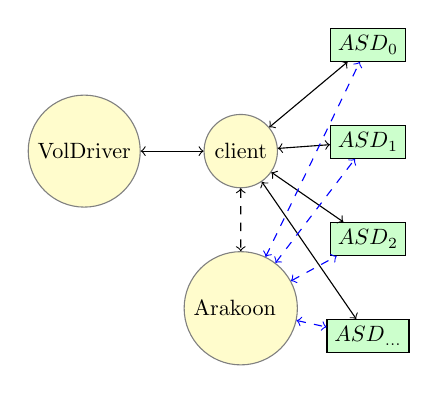
\begin{tikzpicture}[scale = 0.8, transform shape]
        \tikzset{
          my_data/.style={rectangle, fill=green!20, draw},
          my_process/.style={circle, draw = black!50, fill= yellow!20}
        }

        \node (client) [my_process] {client};
        \node (vd)     [my_process, left = of client] {VolDriver};
        \node (nm)     [my_process, below = of client,
                        text width=1.5cm] {Arakoon};
        \node (data0)  [my_data, above right = of client] {$\text{ASD}_0$};
        \node (data1)  [my_data, below = of data0]        {$\text{ASD}_1$};
        \node (data2)  [my_data, below = of data1]        {$\text{ASD}_2$};
        \node (dataX)  [my_data, below = of data2]        {$\text{ASD}_{\ldots}$};

        \path[draw, <->]
        (vd) edge node [left] {} (client)
        ;
        \path[draw, <->]
        (client) edge node [left] {} (data0)
                 edge node [left] {} (data1)
                 edge node [left] {} (data2)
                 edge node [left] {} (dataX)
        ;
        \path[draw, <->, dashed]
        (client) to (nm)
        ;
        \path[draw, <->, dashed, blue]
        (nm) edge node [left] {} (data0)
             edge node [left] {} (data1)
             edge node [left] {} (data2)
             edge node [left] {} (dataX)
        ;
      \end{tikzpicture}

    \end{column}
    \begin{column}[T]{5cm}
      \pause
      \begin{block}{ASD: Alba's Storage Device}
        \begin{itemize}[<+(1)->]
          \item ASD: atomic multi-update (rocksdb)
          \item rpc via capnp
          \item (C++)
        \end{itemize}
      \end{block}
      \pause
      \begin{block}{Arakoon}
        \begin{itemize}[<+(1)->]
          \item 1.8 user hooks
          \item plugin imposing data model
        \end{itemize}
      \end{block}
    \end{column}
  \end{columns}
\end{frame}

\begin{frame}
  \frametitle{Hardware deployment}
  \framesubtitle{Unit of deployment}
  \begin{columns}[T]
    \begin{column}[T]{5cm}
      \begin{block}{1 deployment unit}
      \begin{itemize}
      \item 4x(2TB or 3TB) HDD
      \item 2x 1GbE
      \item 4GB RAM
      \item Dual Atom (Mini-ITX board)
      \item \emph{no hot hdd replacement}
      \end{itemize}
      \end{block}
    \end{column}
    \begin{column}[T]{5cm}
      \begin{block}{Usage}
        \begin{itemize}
          \item unit of replacement.
          \item If 1 disk in a unit fails, work around it.
          \item If 2 disks in a unit fail, consider unit lost.
          \item overhead for 8 units: $(4/3)(8/6)=1.78 $
        \end{itemize}
        \end{block}
    \end{column}
  \end{columns}
\end{frame}

\begin{frame}
  \frametitle{Current Status}
  \framesubtitle{oh boy}
  \begin{itemize}
    \item client lib (C++): features 80\%
    \item client as a proxy (C++, capnp): feature complete
    \item client's client (C++, capnp): VolDriver team
    \item nsm plugin (OCaml): features 80\%
    \item nsm client (C++): object crud only
    \item repair: repair 1 object (+ loop over repair queue)
    \item nsm client (OCaml): feature complete.
    \item asd (C++/OCaml): features 90\%
    \item garbage collection: ongoing
    \item deployment \& mgmt: nowhere.
  \end{itemize}
  Quality: happy path.
\end{frame}
\begin{frame}
  \frametitle{Questions?}
  \framesubtitle{Shoot}
\end{frame}
\end{document}
